\documentclass[12pt,a4paper]{article}
\usepackage[utf8]{inputenc}
\usepackage{amsmath}
\usepackage{graphicx}
\usepackage{subfig}
\usepackage{float}
\usepackage{lipsum}
\usepackage[super]{nth}
\usepackage{hyperref}
\begin{document}
\large
\title{Major Project}
\maketitle
\author{Nrupesh Surya U, Abhinav Basu, Sarvesh Borkar, Ashwani Singh}


%--------------------------------------------------------------------------------
\section*{Abstract}
The problem statement requires a working model for forecasting
the spread of COVID-19 in the United States of America. For this 
project, we will restrict ourselves to New York City which consists of 
5 counties. The data was collected from Official government sources 
as well as private giants such as Google and Apple who collect mobility
data. The dataset collected ranges from March 2020 to April 2021 and contains
27 features which are all time-series data.   
%--------------------------------------------------------------------------------
%--------------------------------------------------------------------------------
\section*{Introduction}
The COVID-19 pandemic, also known as the coronavirus pandemic, is an ongoing global pandemic of coronavirus disease 2019 (COVID-19) caused by severe acute respiratory syndrome coronavirus 2 (SARS-CoV-2).
\\\\
Time series forecasting has been extensively studied using classical 
statistical models like ARIMA, SARIMA and recently developed FBProphet by Facebook.
\\
Time series forecasting can be divided into univariate and multivariate. We will
be focusing on multivariate time series forecasting. 
\\\\
Our goal is to forecast New cases for the city of New York. For this, we transformed our 
time series dataset to a suitable supervised machine learning problem. 

\section*{Data Collection}
Data was collected from the New York City government \href{https://www1.nyc.gov/site/doh/covid/covid-19-data.page}{website}. 
The data collected from this source included new cases, deaths, testing, number of people hospitalized. 
The data had different start dates so the data was merged by removing the missing data and 
thus the time series starts from March, 2020.   
\\\\
Mobility data was collected for the region which had data regarding the movement of people.
The Google mobility data contained features such as residential percent change from baseline,
parks percent change from baseline and so on. These data are location centric which was different
from Apple's Mobility data. This one contained just 3 features : driving, walking and transit which 
were focused just on the means of transportation. 

\section*{Exploratory Data Analysis}
The COVID-19 Cases and Death Counts are visualized in the following plots.
\begin{figure}[H]
    \centering
    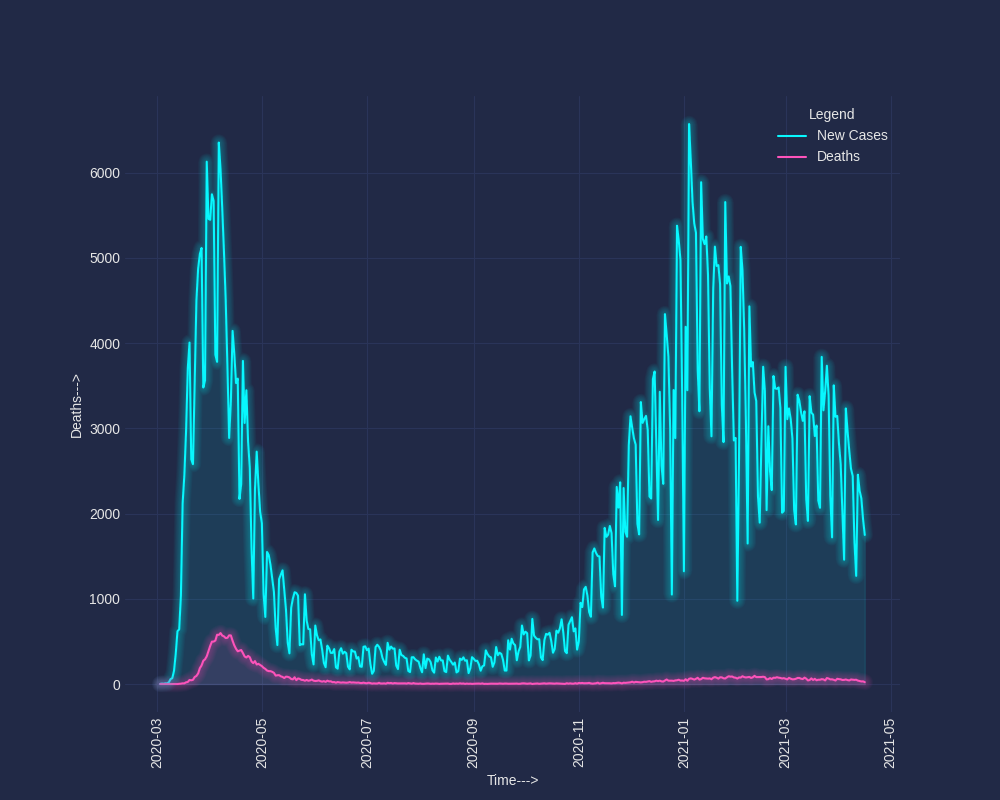
\includegraphics[width=0.75\textwidth,height=75mm]{images/deaths.png}
    \caption{New Cases and Deaths in NYC}
\end{figure}


Figure 1 illustrates the fatality rate and infection rate of COVID-19
and gives a glimplse on exponential growth.

The testing data with splits for positive and antigen testing is shown below.
\begin{figure}[H]
    \centering
    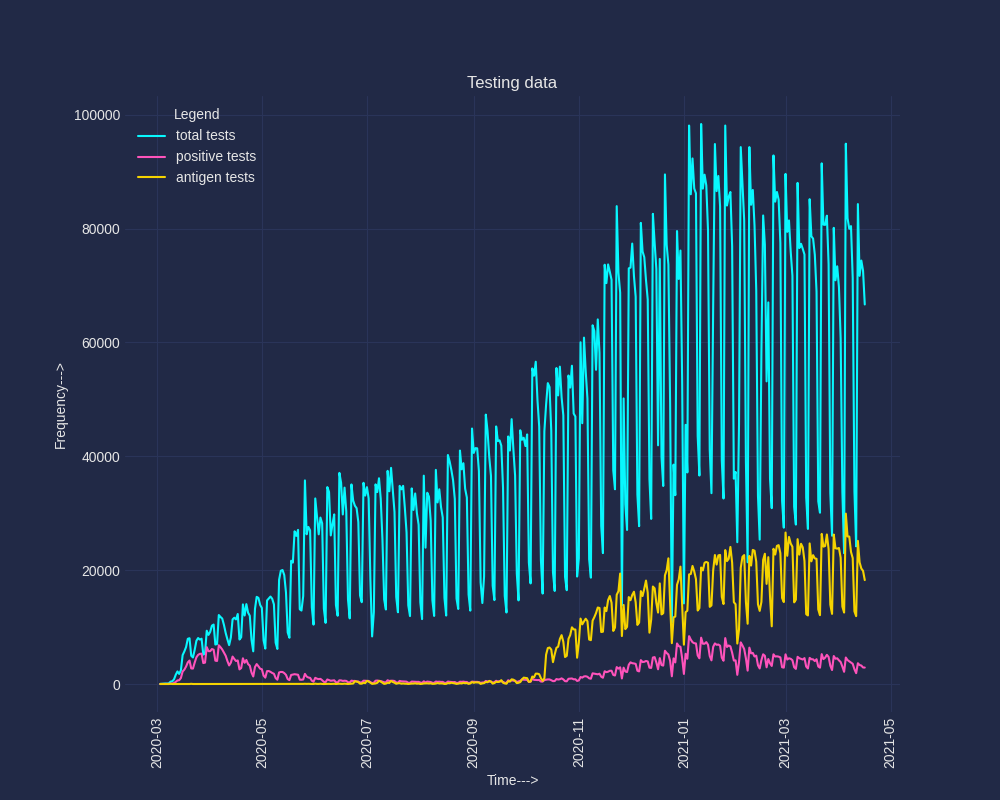
\includegraphics[width=0.75\textwidth,height=75mm]{images/tests.png}
    \caption{Tests, positive tests and antigen tests in NYC}
\end{figure}
Google Mobility contains data which is location
centric such as parks, grocery stories and so on. 
\begin{figure}[H]
    \centering
    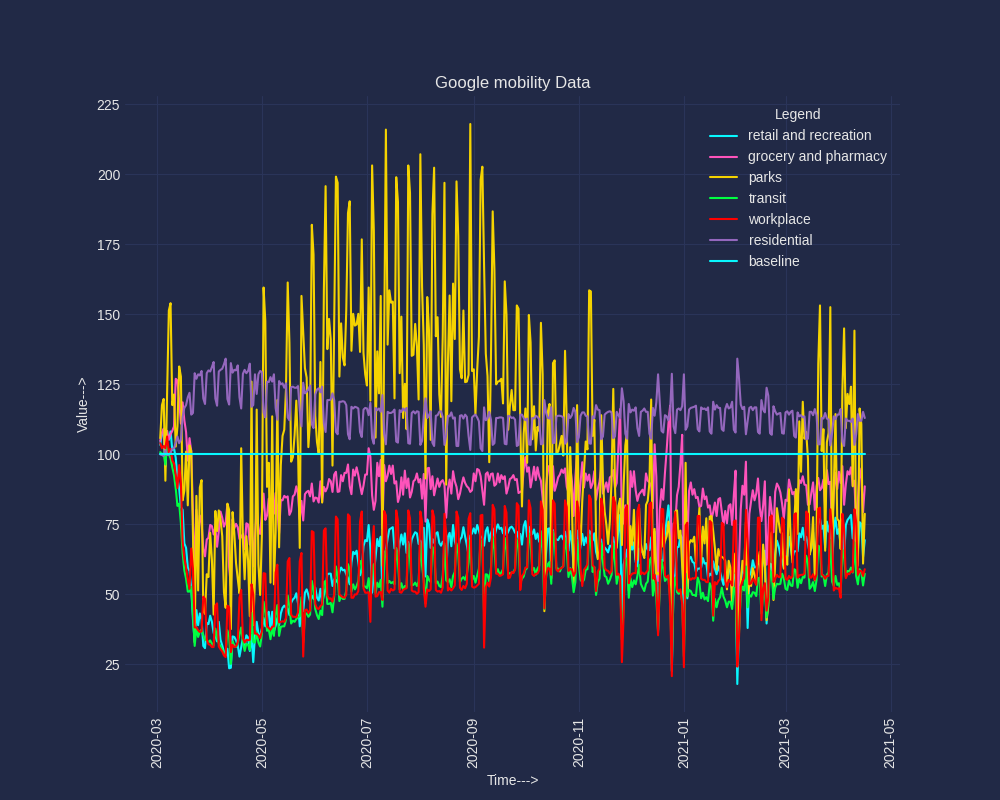
\includegraphics[width=0.6\textwidth,height=60mm]{images/google.png}
    \caption{Google Mobility data}
\end{figure}
From Figure 3, we notice that almost all numbers are down from baseline
except residential, which means people have been staying at home. The other 
exception is Parks where people seemingly visited more than usual after 
lockdown which also plummets down soon enough embracing the second wave.
\\
Meanwhile Apple mobility is more transport oriented and contains driving, walking and transit data.
\begin{figure}[H]
    \centering
    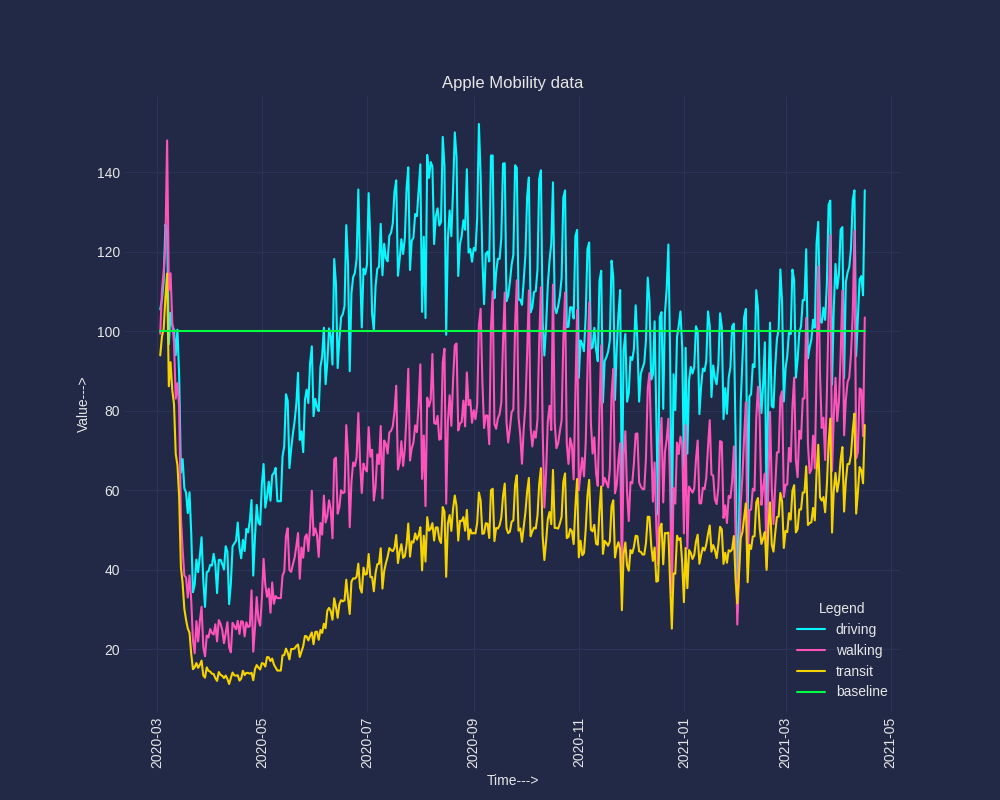
\includegraphics[width=0.6\textwidth,height=60mm]{images/apple.png}
    \caption{Apple Mobility data}
\end{figure}
\section*{Data Representation}
To convert this time series dataset into a supervised machine 
learning problem we use a sliding window method. 
\begin{figure}[H]
    \centering
    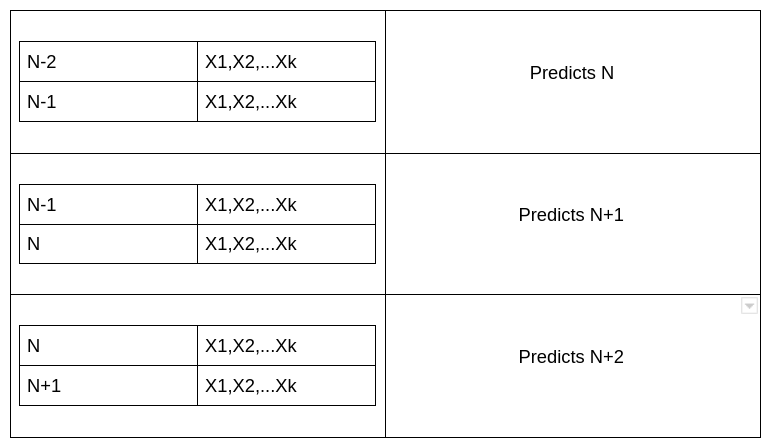
\includegraphics[width=0.6\textwidth,height=60mm]{images/sliding_window.png}
    \caption{Sliding Window with window length 2 which predicts 1 day ahead}
\end{figure}
For instance, in Figure 5, we predict the outcomes of day N using the features of the previous
2 days. 
\\
We need to extend this method to predict days further ahead in the future.
\begin{figure}[H]
    \centering
    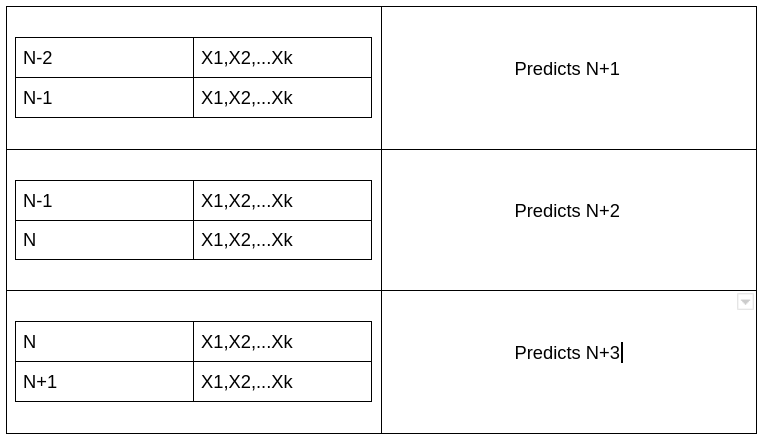
\includegraphics[width=0.6\textwidth,height=60mm]{images/sliding_window_2.png}
    \caption{Sliding Window with window length which predicts 2 days ahead}
\end{figure}
Thus, the window length becomes a hyperparameter which can be tuned further.

\section*{Data Preprocessing}
The entire dataset contained 410 data-points from March-2020 to April-2021. The window 
length was setup to be 7. This meant we had a total of 403 data points usable since we can 
only start predicting from the 7th day. The test data consisted of the last 60 data-points.
The dataset contains 27 columns for each day in the time series.
\\\\
The data was coming from multiple sources and had different
start and end dates. Missing data was removed(only from the beginning and end dates). Mobility data from Google was available county wise and not city wise. For this,
we took the day-wise average of each of the 5 counties in NYC to make up for it. Data was scaled
using standard scalar from Sklearn. Transforming the data into the above-mentioned sliding-window
representation was necessary before the fitting the models.
The training and test datasets further needed transformation from a 3D matrix to a 2D matrix
which was achieved by flattening.

\section*{Models}
The Python library Sklearn was used for obtaining the models which are listed below.
\begin{itemize}
    \item Support Vector Machine : Used for linear and non-linear classification which is 
    benefited by its use of kernel tricks to manipulate data in higher dimensional spaces. 
    Since the number of data points is greater than number of features, SVM can be a good choice for
    this problem. 
    \item ARDRegressor : Automatic Relevance Determination is a classical method
    based on Bayesian interference. It fits the weights of a regression model using an ARD prior. The weights of the regression model are assumed to be in Gaussian distributions.
    \item RandomForestRegressor : Random forest is a decision tree ensemble technique that is capable of mapping complex
    non-linear decision boundaries. It builds a large number of uncorrelated trees so as to
    reduce the amount of variance and improve the accuracy and limit overfitting.
    \item GradientBoostingRegressor : Similar to random forest, gradient boosting is also a decision tree based ensemble
    technique. The difference lies in the principle - gradient boosting uses boosting, where
    the classifiers are trained sequentially, while random forests use bagging, where classifier
    is trained in parallel with a randomised subset of data.
    \item SGDRegressor : SGD stands for Stochastic Gradient Descent where the gradient of the loss is estimated each sample at a time and the model is updated along the way with a decreasing strength schedule (aka learning rate) using 
    either L1 or L2 norm.
    \item LinearRegression : LinearRegression fits a linear model with coefficients to minimize the residual sum of squares between the observed targets in the dataset, and the targets predicted by the linear approximation.\\\\
\end{itemize}
\newpage
\section*{Results and Discussion}

\begin{table}[htb]
    \begin{tabular}{ |c|c|c|c|c|c|c| }
        \hline
         & SVM & ARD & Random Forest & Gradient Boosting & SGD & LR \\
        \hline
        1-day & 0.66977 & 0.48376 & 0.46112 & 0.44985 & 0.56829 & -0.97958 \\
        \hline
        2-day & 0.47136 & 0.54786 & 0.35911 & 0.38275 & 0.24436 & -1.32936 \\
        \hline
        3-day & 0.18115 & 0.28784 & 0.23751 & 0.30467 & -0.15059 & -1.15995 \\
        \hline
        4-day & -0.14321 & 0.06788 & 0.18569 & 0.49359 & 0.06036 & -1.28491 \\
        \hline
        5-day & -0.56157 & 0.02857 & 0.13129 & 0.05533 & -0.42911 & -1.28551 \\
        \hline
        6-day & -0.83036 & -0.12586 & 0.02753 & -0.81896 & -0.84298 & -1.06387 \\
        \hline
        7-day & -0.78608 & 0.27080 & 0.04629 & -1.34171 & -0.48858 & -4.07222 \\
        \hline 
        \end{tabular}
        \caption{ $R^2$ Scores for the models with X-days future predictions}
    \begin{tabular}{ |c|c|c|c|c|c|c| }
        \hline
         & SVM & ARD & Random Forest & Gradient Boosting & SGD & LR \\
        \hline
        1-day & 0.05324 & 0.08323 & 0.08688 & 0.08869 & 0.06960 & 0.31914 \\
        \hline
        2-day & 0.08522 & 0.07289 & 0.10332 & 0.09951 & 0.12182 & 0.37553 \\
        \hline
        3-day & 0.1320  1 & 0.11481 & 0.12292 & 0.11210 & 0.18549 & 0.34822  \\
        \hline
        4-day & 0.18430 & 0.15027 & 0.13128 & 0.08164 & 0.15148 & 0.36836 \\
        \hline
        5-day & 0.25175 & 0.15661 & 0.14005 & 0.15230 & 0.23039 & 0.36846 \\
        \hline
        6-day & 0.29508 & 0.18150 & 0.15678 & 0.29324 & 0.29712 & 0.33273 \\
        \hline
        7-day & 0.28794 & 0.11756 & 0.15375 & 0.37752 & 0.23998 & 0.81772 \\
        \hline 
        \end{tabular}
        \caption{MSE Scores for the models with X-days future predictions}
    \begin{tabular}{ |c|c|c|c|c|c|c| }
        \hline
         & SVM & ARD & Random Forest & Gradient Boosting & SGD & LR \\
        \hline
        1-day & 0.17615 & 0.22720 & 0.24284 & 0.24944 & 0.21999 & 0.42545 \\
        \hline
        2-day & 0.23663 & 0.21202 & 0.25754 & 0.24614 & 0.29486 & 0.50959 \\
        \hline
        3-day & 0.30005 & 0.27463 & 0.28711 & 0.27406 & 0.37590 & 0.47509  \\
        \hline
        4-day & 0.36192 & 0.30748 & 0.30318 & 0.21971 & 0.33656 & 0.51561 \\
        \hline
        5-day & 0.25175 & 0.15661 & 0.14005 & 0.15230 & 0.23039 & 0.36846 \\
        \hline
        6-day & 0.47013 & 0.32341 & 0.32719 & 0.46402 & 0.46736 & 0.44117 \\
        \hline
        7-day & 0.46838 & 0.28463 & 0.31675 & 0.53654 & 0.41017 & 0.71479 \\
        \hline 
        \end{tabular}
        \caption{MAE Scores for the models with X-days future predictions}
\end{table}
\newpage
\begin{itemize}
    \item $R^2$ score : Best possible score is 1.0 and it can be negative (because the model can be arbitrarily worse). A constant model that always predicts the expected value of y, disregarding the input features, would get a score of 0.0.
        \begin{equation}
            R^2 = 1 - \frac{\sum_{i=1}^{n}(y_i - \tilde{y_i})^2}{\sum_{i=1}^{n}(y_i - \bar{y})^2} 
        \end{equation}
    \item MSE score : Mean Squared Error measures the average of the squares of the errors—that is, the average squared difference between the estimated values and the actual value. 
        \begin{equation}
            MSE = \frac{1}{n}\sum_{i=1}^{n}(y_i - \tilde{y_i})^2
        \end{equation}
    \item MAE score : Mean Absolute Error is a measure of errors between paired observations expressing the same phenomenon
    \begin{equation}
        MAE = \frac{1}{n}\sum_{i=1}^{n}|y_i - \tilde{y_i}|
    \end{equation}
\end{itemize}

The trends from Table 1,2 and 3 suggest that as we increase the prediction period, 
the error shoots up significantly. SVM seems to be performing best for predicting 
1 day ahead, while other models (except LR) perform better in the later stages.
\newpage
\begin{figure}[H]
    \centering
    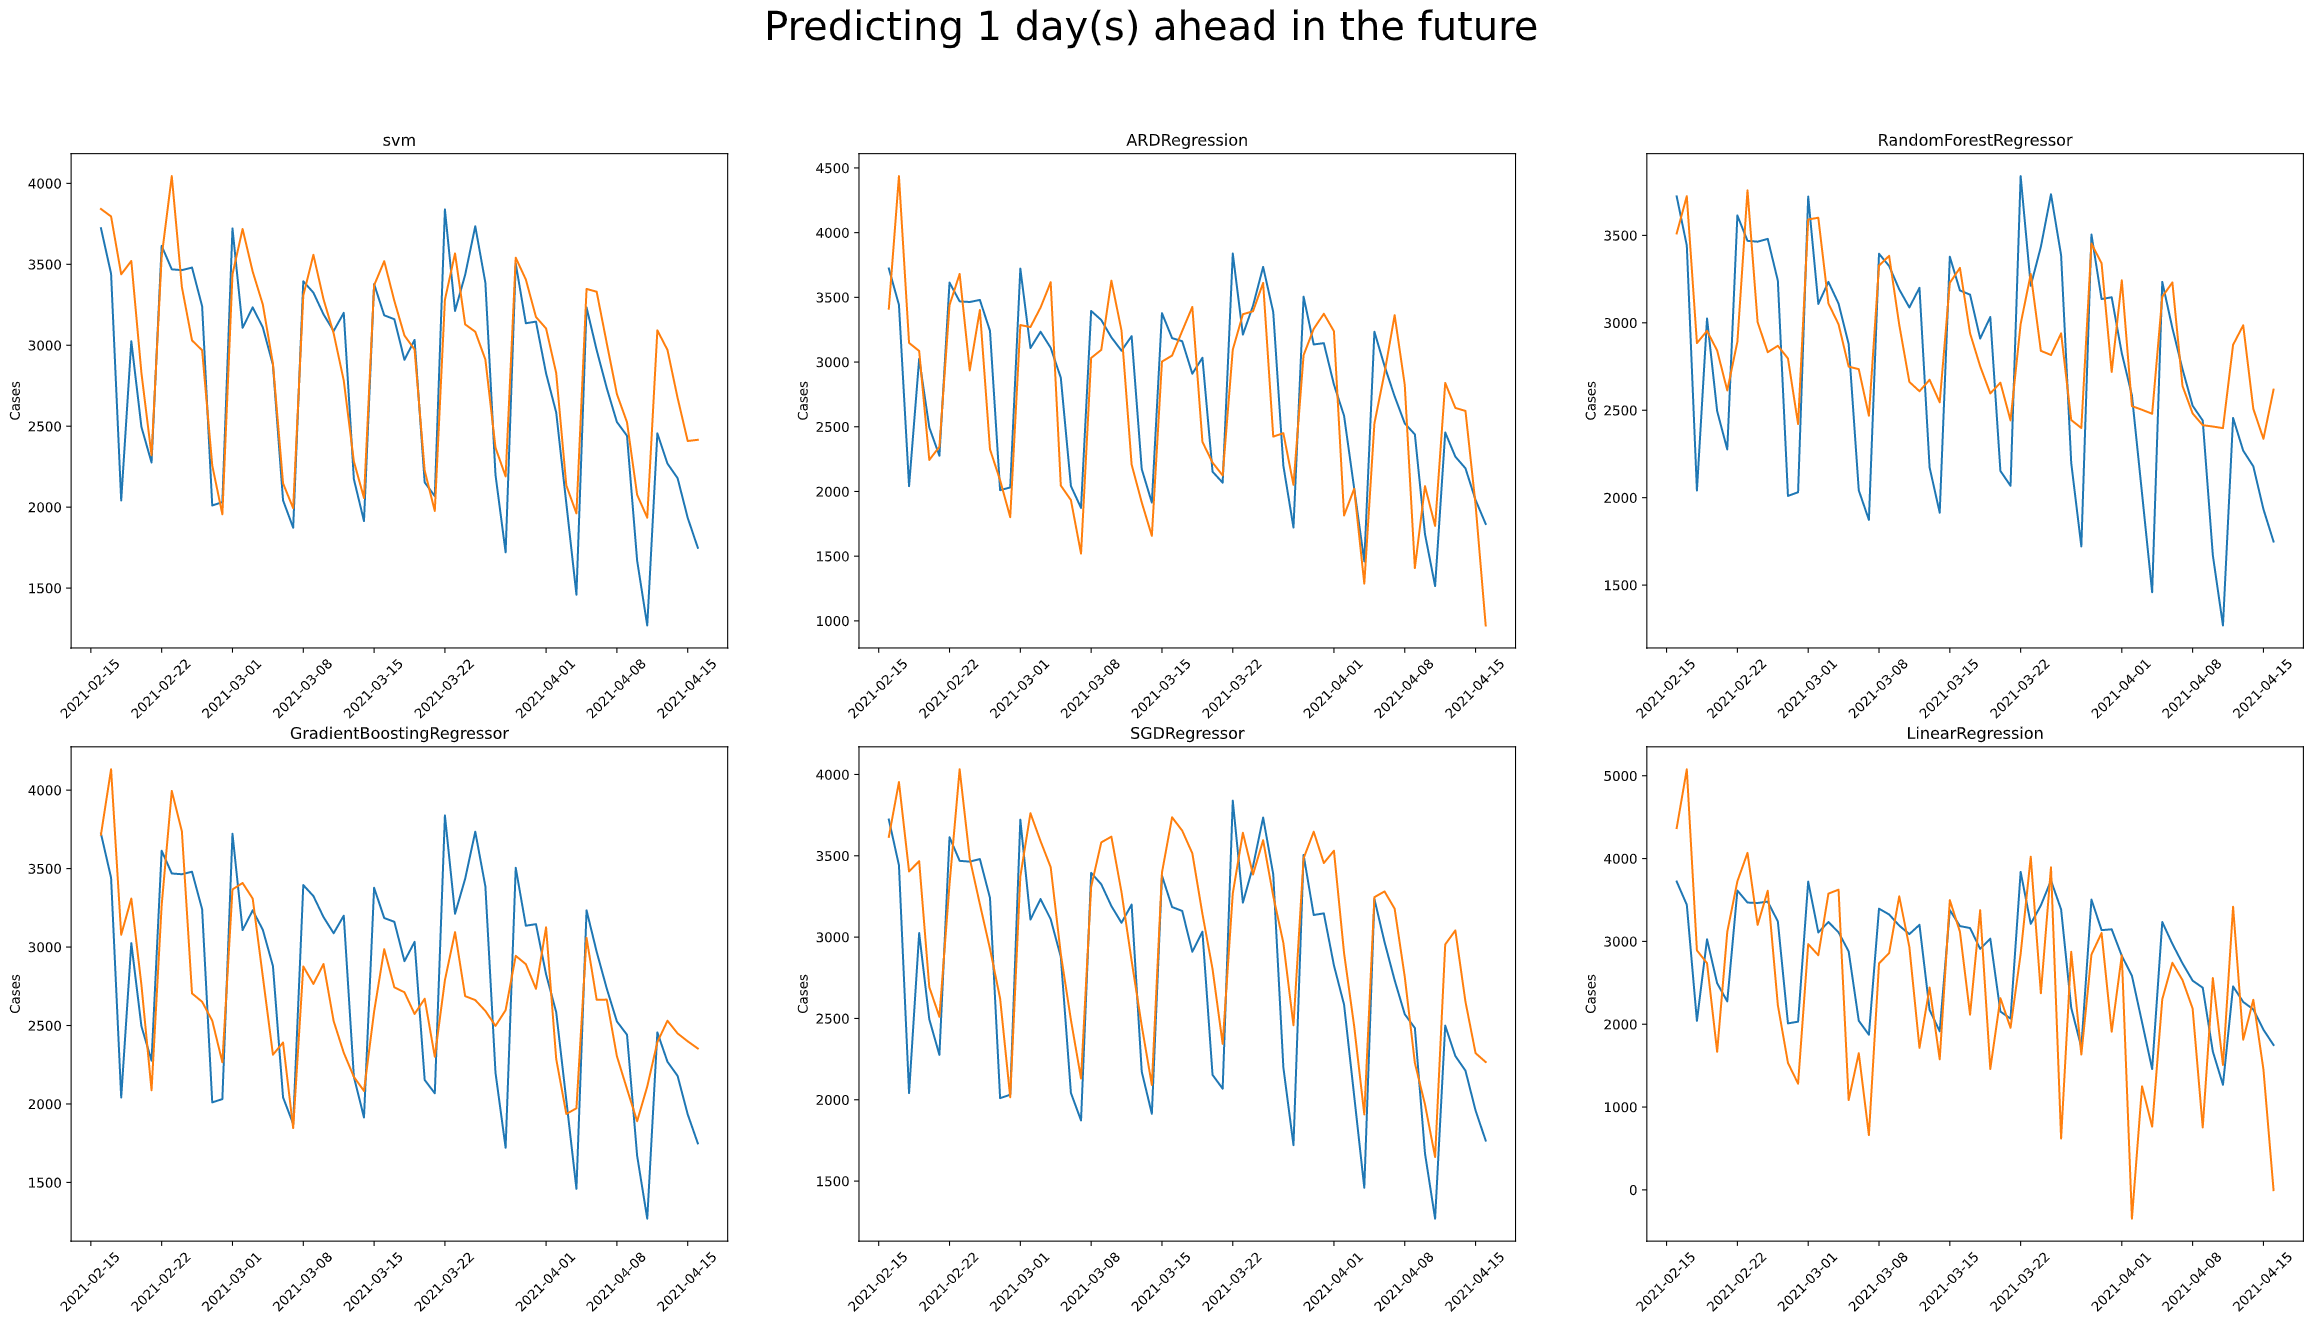
\includegraphics[width=1\textwidth,height=80mm]{images/1_day.png}
    \caption{Prediction vs Test data when predicting 1 day ahead}
\end{figure}

\begin{figure}[H]
    \centering
    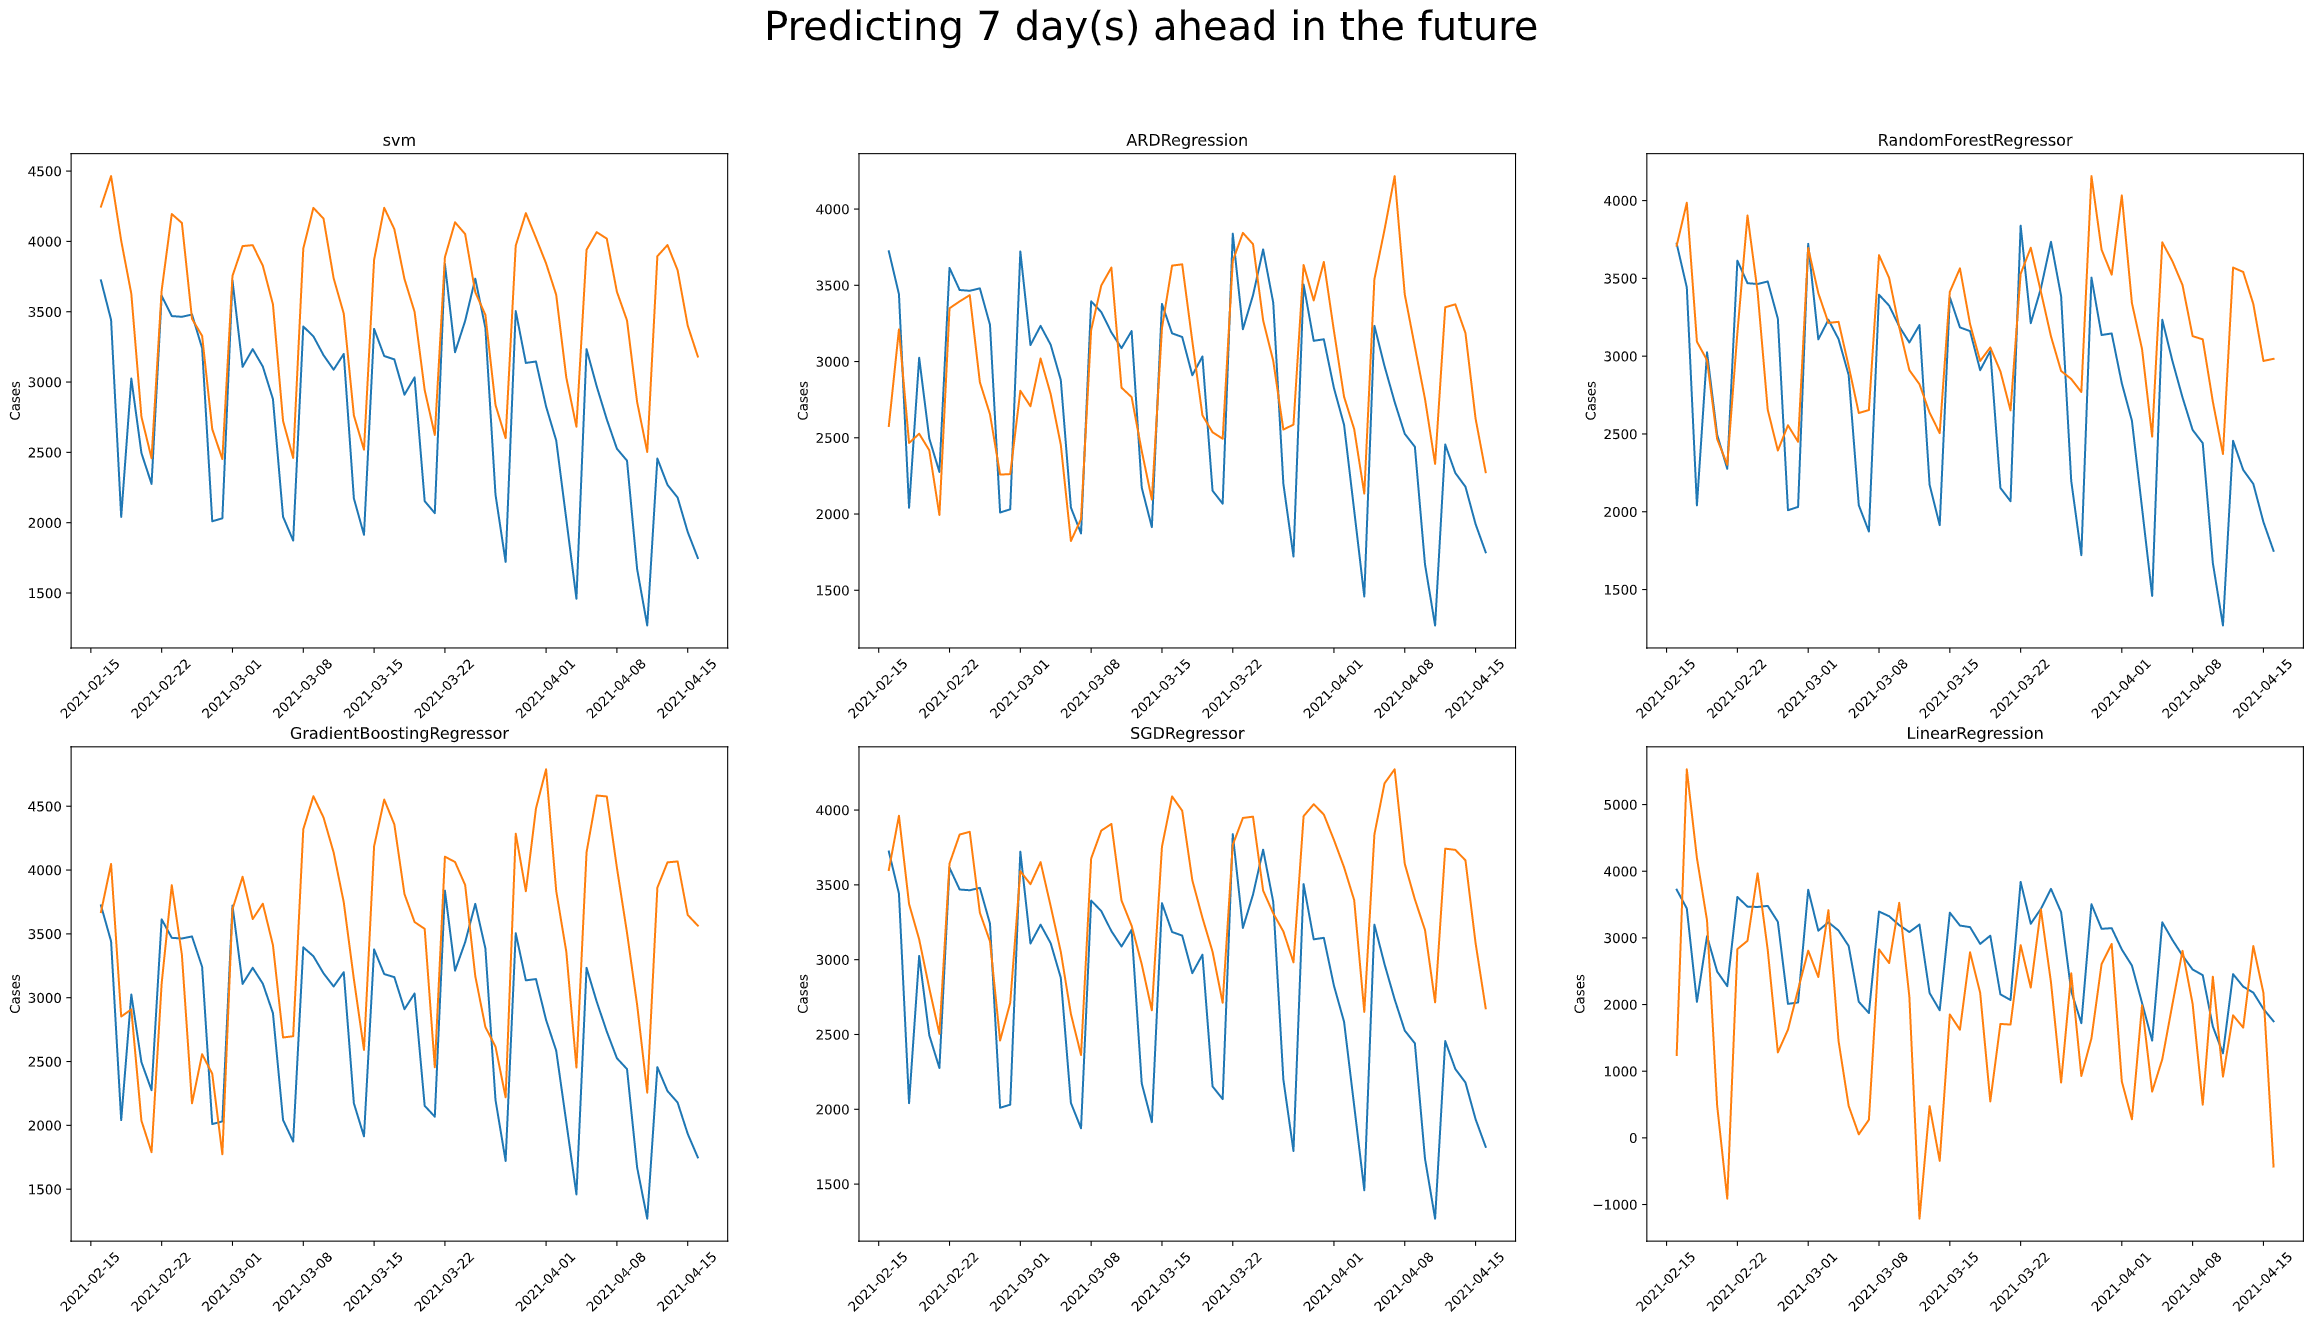
\includegraphics[width=1\textwidth,height=80mm]{images/7_day.png}
    \caption{Prediction vs Test data when predicting 7 days ahead}
\end{figure}
The stark contrast in prediction shows how bad the models perform over time. 
\section*{Comparison with statistical models}

\end{document}